\documentclass[a4paper,12pt]{article}
\usepackage{mypreamble}

%% Page setup
\geometry{
    margin=2cm,
    includehead,
    % includefoot,
    headsep=\baselineskip,
}
\pagestyle{fancy}
\fancyfoot{}
\MakeDoubleHeader% {<l1>}{<l2>}{<r1>}{<r2>}
    {\TextHomeworkEng~\#4}
    {Boolean Algebra}
    {\TextDiscreteMathEng}
    {\IconFall~Fall 2021}

%% Add custom setup below

\begin{document}

\selectlanguage{english}

\begin{tasks}
    \item Perform the following steps:
    \begin{subtasks}
        \item Calculate the SHA-256 hash~$h$ of the string $s = \verb|"Your Full Name HW4"|$ (substitute your full name as in the scores table, without quotes, with all spaces, encoded in UTF-8).
        Convert hash~$h$ to a 256-bit binary string~$b$ (prepend leading zeros if necessary).
        Cut the binary string~$b$ into eight 32-bit slices $r_1, \dotsc, r_8$.
        Xor all slices into 32-bit string $d = r_1 \xor \dotsb \xor r_8$.

        \item Draw the Karnaugh map (see a template below) for a function $f(A,B,C,D,E)$ defined by the truth table~$d$ (MSB corresponds to~$\vvmathbb{0}$, LSB to~$\vvmathbb{1}$).
        Use it to find the minimal~DNF.

        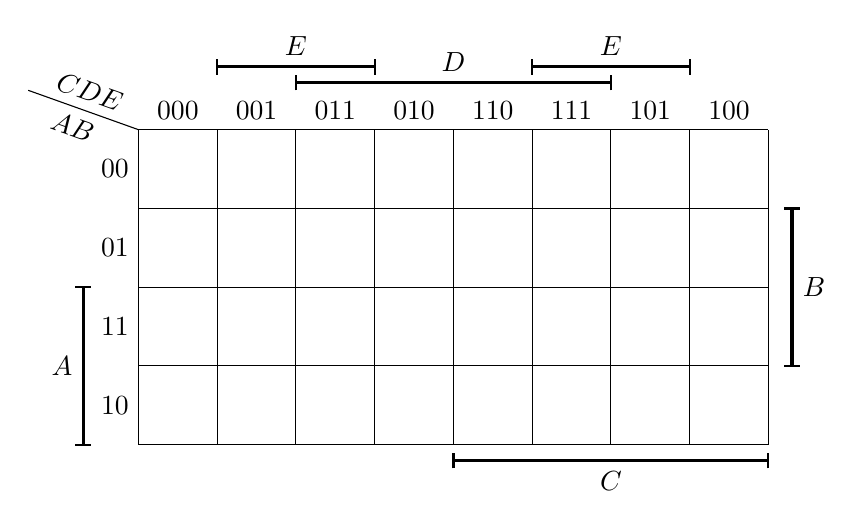
\begin{tikzpicture}[]
            \def\sidelinepaw{0.1}
            \newcommand\sidelineV[4]{% {<start>}{<height>}{<node-style>}{<node-text>}
                \coordinate (start) at #1;
                \draw[thick] (start) +(-\sidelinepaw,0) -- +(\sidelinepaw,0);
                \draw[thick] (start)++(0,#2) +(-\sidelinepaw,0) -- +(\sidelinepaw,0);
                \draw[very thick] (start) -- node[#3]{#4} ++(0,#2);
            }
            \newcommand\sidelineH[4]{% {<start>}{<width>}{<node-style>}{<node-text>}
                \coordinate (start) at #1;
                \draw[thick] (start) +(0,-\sidelinepaw) -- +(0,\sidelinepaw);
                \draw[thick] (start)++(#2,0) +(0,-\sidelinepaw) -- +(0,\sidelinepaw);
                \draw[very thick] (start) -- node[#3]{#4} ++(#2,0);
            }

            \draw (0,0) grid (8,4);
            \node[above] at (0.5,4) {000};
            \node[above] at (1.5,4) {001};
            \node[above] at (2.5,4) {011};
            \node[above] at (3.5,4) {010};
            \node[above] at (4.5,4) {110};
            \node[above] at (5.5,4) {111};
            \node[above] at (6.5,4) {101};
            \node[above] at (7.5,4) {100};
            \node[left] at (0,0.5) {10};
            \node[left] at (0,1.5) {11};
            \node[left] at (0,2.5) {01};
            \node[left] at (0,3.5) {00};
            \draw (0,4) -- node[sloped,below]{$AB$~~} node[sloped,above]{$CDE$} ++(-1.4,.5);

            % \draw[very thick] (-0.7,0) -- node[left]{$A$} ++(0,2);
            % \draw[very thick] (8.3,1) -- node[right]{$B$} ++(0,2);
            % \draw[very thick] (4,-0.2) -- node[below]{$C$} ++(4,0);
            % \draw[very thick] (2,4.6) -- node[above]{$D$} ++(4,0);
            % \draw[very thick] (1,4.8) -- node[above]{$E$} ++(2,0);
            % \draw[very thick] (5,4.8) -- node[above]{$E$} ++(2,0);
            \sidelineV{(-0.7,0)}{2cm}{left}{$A$}
            \sidelineV{(8.3,1)}{2}{right}{$B$}
            \sidelineH{(4,-0.2)}{4}{below}{$C$}
            \sidelineH{(2,4.6)}{4}{above}{$D$}
            \sidelineH{(1,4.8)}{2}{above}{$E$}
            \sidelineH{(5,4.8)}{2}{above}{$E$}
        \end{tikzpicture}
        \vspace{-5mm}
    \end{subtasks}


\makeatletter
\newtcolorbox{notebox}[1][]{%
    enhanced jigsaw, % better frame drawing
    borderline west={1pt}{0pt}{black}, % straigh vertical line at the left edge
    sharp corners, % no rounded corners
    boxrule=0pt, % no real frame,
    % fonttitle={\large\bfseries},
    fonttitle={\bfseries},
    coltitle={black},  % Black colour for title
    title={Note:\ },  % Fixed title
    attach title to upper, % Move the title into the box,
    % right=0pt,
    top=0pt,
    bottom=0pt,
    frame hidden,
    baseline={\tcb@height-2\kvtcb@boxsep+\baselineskip-2\lineskip},
    #1
}
\makeatother

    \item For each given function $f_i$ of 4 arguments, draw the Karnaugh map and use it to find BCF, minimal DNF, and minimal CNF. Additionally, construct ANF (Zhegalkin polynomial) using either the \enquote{triangle} (tabular) method or the Pascal method (use each method at least once).

    \begin{notebox}
    \RaggedRight
    WolframAlpha interprets the query \enquote{$n$-th Boolean function of $k$ variables} in a reverse manner, \ie it produces a function with a reversed truth table. In order to employ WolframAlpha properly, manually flip the truth table, \eg the correct query for $f^{2}_{10}$ would be \enquote{5th~Boolean function of 2~variables}, since $\texttt{rev}(1010_2) = 0101_2 = 5_{10}$.
    \end{notebox}

    \begin{multicols}{2}
    \begin{subtasks}
        \item $f_{\arabic{subtasksi}} = f^{4}_{47541}$
        \item $f_{\arabic{subtasksi}} = \sum m (1,4,5,6,8,12,13)$
        \item $f_{\arabic{subtasksi}} = f^{4}_{51011} \xor f^{4}_{40389}$
        \item $f_{\arabic{subtasksi}} = A\overline{B}D + \overline{A}\,\overline{C}D + \overline{B}C \overline{D} + A\overline{C}D$
    \end{subtasks}
    \end{multicols}


    \item Convert the following formulae to CNF.

    \begin{multicols}{2}
    \begin{subtasks}
        \item $X \iff (A \land B)$
        \item $Z \iff \biglornolim{\!i} C_i$
        \item $R \implies (S \implies (T \implies \biglandnolim{i} F_i))$
        \item $M \implies (H \iff \biglornolim{\!i} D_i)$
    \end{subtasks}
    \end{multicols}


\tcbset{
    dang/.style={
        enhanced,
        breakable,
        fonttitle=\bfseries,
        before skip=2mm,
        after skip=2mm,
        colframe=blue!40!black,
        colback=white,
        colbacktitle=blue!40!black,
        boxrule=0.5mm,
        arc is angular,
        attach boxed title to top left={
            xshift=1cm,
            yshift*=1mm-\tcboxedtitleheight
        },
        varwidth boxed title*=-3cm,
        boxed title style={
            frame code={
                \path[fill=tcbcolback!30!black]
                    ([yshift=-1mm,xshift=-1mm]frame.north west)
                    arc[start angle=0,end angle=180,radius=1mm]
                    ([yshift=-1mm,xshift=1mm]frame.north east)
                    arc[start angle=180,end angle=0,radius=1mm];
                \path[left color=tcbcolback!60!black,
                      right color=tcbcolback!60!black,
                      middle color=tcbcolback!80!black]
                    ([xshift=-2mm]frame.north west) -- ([xshift=2mm]frame.north east)
                    [rounded corners=1mm]-- ([xshift=1mm,yshift=-1mm]frame.north east)
                    -- (frame.south east) -- (frame.south west)
                    -- ([xshift=-1mm,yshift=-1mm]frame.north west)
                    [sharp corners]-- cycle;
            },
            interior engine=empty,
        },
    },
}

\newtcolorbox{defbox}[2][]{% [<style>]{<title>}
    dang,
    title={#2},
    #1
}

    \item Prove rigorously the following theorem.

    \begin{defbox}{Post's Functional Completeness Theorem}
        A system $F$ of boolean functions is functionally complete (\ie $F^{*} = \mathbb{F}$) \emph{iff} for each of the five defined classes $T_0$, $T_1$, $S$, $M$, $L$, there is a function $f \in F$ which does not belong to that class.
    \end{defbox}


    \item For each given system of functions $F_i$, determine whether it is functionally complete.
    For each basis $F_i$, use it to rewrite the function $g(A,B,C) = A \implies ((\neg A \xor B) \land \neg C)$.
    Draw a schema of it.

    \begin{multicols}{2}
    \begin{subtasks}
        \item $F_{\arabic{subtasksi}} = \Set{ \land, \lor, \neg }$
        \item $F_{\arabic{subtasksi}} = \Set{ f^{2}_{14} }$
        \item $F_{\arabic{subtasksi}} = \Set{ \implies, \centernot\implies }$
        \item $F_{\arabic{subtasksi}} = \Set{ 1, \iff , \land }$
    \end{subtasks}
    \end{multicols}

    % \item \ldots
\end{tasks}
\end{document}
